\documentclass[journal]{IEEEtran}
\usepackage[a5paper, margin=10mm]{geometry}
%\usepackage{lmodern} % Ensure lmodern is loaded for pdflatex
\usepackage{tfrupee} % Include tfrupee package


\setlength{\headheight}{1cm} % Set the height of the header box
\setlength{\headsep}{0mm}     % Set the distance between the header box and the top of the text


%\usepackage[a5paper, top=10mm, bottom=10mm, left=10mm, right=10mm]{geometry}

%
\usepackage{float}
\usepackage{pythontex}
\usepackage{graphicx}
\usepackage{gensymb}
\usepackage{gvv-book}
\usepackage{gvv}
\setlength{\intextsep}{10pt} % Space between text and floats

\makeindex

\begin{document}
\bibliographystyle{IEEEtran}
\onecolumn
\newpage
\title{Assignment-2}
\author{AI24BTECH11002 - K.AKSHAY TEJA}
\maketitle




\section{Vector Arithmetic}
\begin{enumerate}
 \item If the coordinates of points $\vec{A}$ and $\vec{B}$ are \brak{-2,-2} and \brak{2,-4} respectively, find the coordinates of $\vec{P}$ such that $AP = \frac{3}{7} AB$, and $\vec{P}$ lies on the line segment $AB$. 
 
    \hfill {(10, 2015)}

 \solution
 Given, coordinates of $\vec{A}$ are \brak{-2,-2} and coordinates of $\vec{B}$ are \brak{2,-4}.$\vec{P}$ divides $\vec{AB}$ in ratio 3:4.So, k=$\frac{3}{4}$
 \begin{align*}
	 \implies \vec{P} &= \frac{\frac{3}{4}\vec{B} + \vec{A}}{\frac{3}{4} + 1} \tag{Setion Formula}\\
	 &= \myvec{\frac{-2}{7}\\\frac{-20}{7}} 
 \end{align*}
		\begin{figure}[h]    
	  \begin{center}
		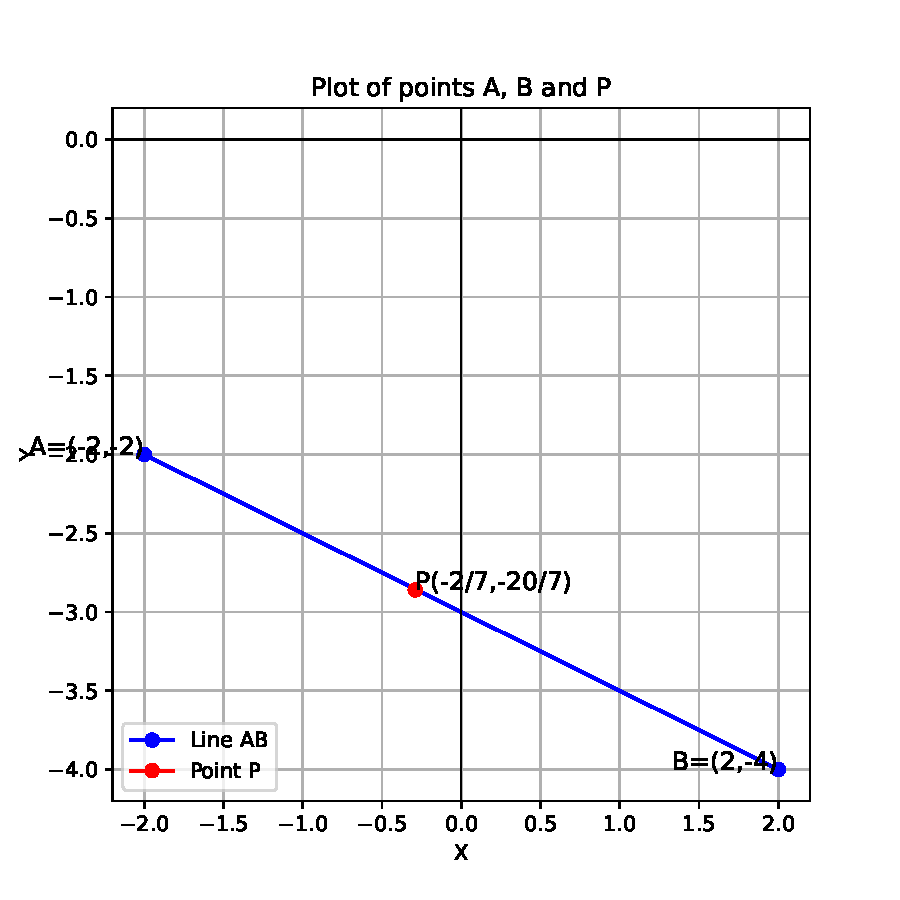
\includegraphics[width=0.8\textwidth]{Fig.pdf}
	 \end{center}	  
	\end{figure}
\end{enumerate}
\end{document}

